%------------------------------- CHAPTER NAME --------------------------------
\chapter{Take-off performance}
Although the take-off field length may seem like a performance characteristic of secondary importance, it is very often one of the critical design constraints. If the required runway length is too long, the aircraft cannot take-off with full fuel or full payload and its economics are compromised.

Take-off performance plays so a significant role in the preliminary design of an aircraft because it is both a requirement, specified by the FAR and by the customer, to be fulfilled, both a driving parameter in the definition of the design point. 

%-------------------------- THEORETICAL BACKGROUND ---------------------------
\section{Theoretical background}
The takeoff may be considered as made up of two parts: a ground run and an air run, as shown schematically in figure~\ref{fig:TOrun}. The simplest description of the take-off process is that the engine thrust is increased to the takeoff level at x = 0 and the brakes are released to begin acceleration down the runway. At some point, the pilot commands rotation of the aircraft which lifts the nose wheel from the ground and allows to achieve the takeoff angle of attack; in this way the aircraft lift can grows faster and, when it is equal to the aircraft maximum take-off weight, the aircraft can lifts completely from the ground and begins climbing. The point at which it reaches an altitude of 35 \si{ft} (10.7 \si{\meter}), is considered, for an aircraft which refers to the FAR-25, the end of the take-off run. 

This is the usual situation for take-off; subsequently, the modifications to safely deal with a takeoff emergency, such as an engine failure, will be discussed.

\begin{figure}[!t]
\centering
\includegraphics[keepaspectratio, width=1.02\textwidth]{TakeOffRun}
\caption{Scheme of an aircraft take-off run}
\label{fig:TOrun}
\end{figure}

%-----------------------------AOE Take-Off subsection-----------------------------
\subsection{\gls{acr:AOE} take-off run}
In order to deal with the calculation of the take-off run distance, a smart strategy is to find out all the foundamentals variables, which describes completely the aircraft state in this phase, and so, to study the dynamic system in exam in a state-space representation.

\noindent
To find out these state variables it is necessary to analyze aircraft equations of motion during take-off phases, these latter described as follows.
\begin{itemize}
\item \textbf{Ground roll phase}: starting from standstill with brakes released and at maximum power output, the aircraft accelerates on the runway, with constant angle of attack, until it reaches a speed equals to the rotation speed V\textsubscript{Rot}; after that the following subphase begin.

\begin{itemize}
\item \textbf{Rotation phase}: a short phase in which the pilot gives an assigned pitching law to lift the aircraft nose and, as a result, increasing the angle of attack. This phase ends when the load factor is equal to 1, meaning that the lift has reached the value of the maximum take-off weight, and the relative lift-off speed is indicated with V\textsubscript{LO}. 

\end{itemize}

\item \textbf{Airborne phase}: is the phases in which the aircraft, once it has lifted from the ground, gains altitude until it reaches the obstacle height of 35 \si{ft} (10.7 \si{\meter}) imposed by the FAR-25. This phase begin at V\textsubscript{LO} and ends at the speed related to the obstacle overcoming, indicated with V\textsubscript{2}; furthermore it can be divided into the followngs two subphases:

\begin{itemize}
\item \textbf{Transition phase}: in which the aircraft rotates in order to increase the climb angle ($\gamma$) with the result of increasing the angle of attack and the relative lift coefficient, which should not surpass a safety value of the 90\% of the maximumlift coefficient in take-off configuration. This sub-phase ends when the desidered climb speed is reached.

\item \textbf{Climb-out to the obstacle phase}: in which the aircraft climbs at constant climb angle until the obstacle is surpassed.
\end{itemize}
\end{itemize}

\noindent
For more information regarding take-off equations of motion during each of the previously described phases, the reader can refer to~\cite{McCormick}.

\bigskip
\noindent
The set of \gls{acr:ODE} that models the take-off run is written in the following form:

\begin{equation}\label{eq:Take:Off:System:Dynamics:A}
    \LEFTRIGHT\lcbrace\rcbrace{\begin{array}{c}\dot{s}\\[2pt] \dot{V} \\[2pt] \dot{\gamma} \\[2pt] \dot{h} \end{array}}
= 
    \LEFTRIGHT\lcbrace\rcbrace{\begin{array}{l}
       f_1 \big(\, s,\, V,\, \gamma,\, h \,; \, \alpha \big) \\[4pt]
       f_2 \big(\, s,\, V,\, \gamma,\, h \,; \, \alpha \big) \\[4pt]
       f_3 \big(\, s,\, V,\, \gamma,\, h \,; \, \alpha \big) \\[4pt]
       f_4 \big(\, s,\, V,\, \gamma,\, h \,; \, \alpha \big)
    \end{array}}
\qquad
    \text{with}\quad
    \LEFTRIGHT\lcbrace.{\begin{array}{l} x_1 = s\\[2pt] x_2 = V \\[2pt] x_3 = \gamma \\[2pt] x_4 = h \end{array}}
\qquad
    \text{and}\quad
    u = \alpha
\end{equation}

\noindent
These equations can be also written in a more concisely way as shown below.

\begin{equation}
\label{eq:Take:Off:System:Dynamics:B}
\dot{\vec{x}} = \vec{f}\big(\, \vec{x}\,;\,u \,\big)
\end{equation}

\noindent
The unknown $\vec{x} = [\mspace{2mu} x_1,\, x_2,\, x_3,\, x_4 \mspace{2mu}]^{\text{T}}$ is the vector of state variables. The input $u(t)$ is a given function of time, for $0 \leq t \leq t_{\text{final}}$, that corresponds to an assumed time history of the angle of attack during take-off.

The right-hand sides of system (\ref{eq:Take:Off:System:Dynamics:A}) are defined by the following functions:

\begin{subequations}\label{eq:Take:Off:System:Dynamics:RHS:functions}
\begin{equation}\label{eq:Take:Off:System:Dynamics:RHS:functions:A}
f_1 \big(\, \vec{x}\,,\,u \,\big) =  x_2
\end{equation}

\begin{equation}\label{eq:Take:Off:System:Dynamics:RHS:functions:B}
f_2 \big(\, \vec{x}\,,\,u \,\big) =
  \frac{g}{W}
    \LEFTRIGHT\lcbrace.{
      \begin{array}{l@{\rule{2em}{0pt}}l} 
        T(x_2) - D(x_2,u) - \mu \big[ W - L(x_2,u) \big]
          & \text{if} \;\, \mathcal{S}(x_2 , u) < 1
        \\[1em]
        T(x_2) \cos u - D(x_2,u) - W \sin x_3
          & \text{if} \;\, \mathcal{S}(x_2 , u) \geq 1
      \end{array}
    }  
\end{equation}

\begin{equation}\label{eq:Take:Off:System:Dynamics:RHS:functions:C}
f_3 \big(\, \vec{x}\,,\,u \,\big) =
  \frac{g}{W\,x_2}
    \LEFTRIGHT\lcbrace.{
      \begin{array}{l@{\rule{2em}{0pt}}l} 
        0
          & \text{if} \;\, \mathcal{S}(x_2 , u) < 1
        \\[1em]
        L(x_2,u) + T(x_2)\sin u - W \cos x_3
          & \text{if} \;\, \mathcal{S}(x_2 , u) \geq 1
      \end{array}
    }  
\end{equation}

\begin{equation}\label{eq:Take:Off:System:Dynamics:RHS:functions:D}
f_4 \big(\, \vec{x}\,,\,u \,\big) =  x_2 \, \sin x_3
\end{equation}

\noindent
The thrust $T(x_2)$ is calculated by means of the interpolating function $T_{\text{tab}}\big(V_{\text{a}}\big)$ based on a table lookup algorithm, where $V_{\text{a}} = V + V_{\text{w}}$ is the airspeed and $V_{\text{w}}$ is the wind speed (horizontal component, positive if opposite to the aircraft motion).

The drag $D$ and lift $L$, as functions of airspeed $V_{\text{a}}$ and angle of attack, are given by the following conventional formulas.

\begin{equation}\label{eq:Take:Off:System:Dynamics:RHS:functions:E}
D(x_2,u) = \frac{1}{2} \, \rho \, \big( x_2 + V_{\text{w}}\cos x_3 \big)^2 \,S \, C_D\big( u \big)
\end{equation}

\begin{equation}\label{eq:Take:Off:System:Dynamics:RHS:functions:E}
L(x_2,u) = \frac{1}{2} \, \rho \, \big( x_2 + V_{\text{w}}\cos x_3 \big)^2 \,S \, C_L\big( u \big)
\end{equation}

\noindent
The switching function $\mathcal{S}$ of aircraft velocity and angle of attack is defined as follows:

\begin{equation}\label{eq:Take:Off:System:Dynamics:RHS:functions:D}
\mathcal{S}(x_2 , u) = \frac{L(x_2,u)}{W \cos x_3}
\end{equation}
\end{subequations}

\noindent
The formulas (\ref{eq:Take:Off:System:Dynamics:RHS:functions}) make the system (\ref{eq:Take:Off:System:Dynamics:B})  a closed set of ODEs.

\noindent
When the function $u(t)$ is assigned and the system is associated to a set of initial conditions, in this particular case equal to $\vec{x}_0 = [\mspace{2mu} 0,\, 0,\, 0,\, 0 \mspace{2mu}]^{\text{T}}$, a well-posed \gls{acr:IVP} is formed, which can be solved numerically.

The function $u$ can be constructed by picking the time $t_{\text{Rot}}$ when the rotation speed $V_{\text{Rot}}$ is reached along the ground roll. It is assumed that

\begin{equation}\label{eq:Take:Off:System:Dynamics:Alpha:Law}
u (t) =
    \LEFTRIGHT\lcbrace.{
      \begin{array}{l@{\rule{2em}{0pt}}l} 
        \alpha_{\text{g}}
          & \text{if} \;\, t < t_{\text{Rot}}
        \\[1em]
        \alpha_1(t)
          & \text{if} \;\, t \geq t_{\text{Rot}}
      \end{array}
    }
\end{equation}

with a constant $\alpha_{\text{g}}$ during the ground run up to the rotation speed, and a given non-zero law $\alpha_1(t)$ for the post-rotation angle of attack time history. 

In table~\ref{tab:Take:Off:Speeds:FAR25} are reported the take-off characteristic speeds and their corresponding requirements as defined by FAR~25.

\begingroup
\centering
\begin{longtable}[H]{lll}
\label{tab:Take:Off:Speeds:FAR25}\\
\toprule
Speed & Description & Requirement
\\ \midrule
\endfirsthead

\multicolumn{3}{l}%
  {\relsize{-1}({\itshape continued from previous page})}\\
\toprule
Speed & Description & Requirement
\\ \midrule
\endhead

\midrule \multicolumn{3}{r}{{\relsize{-1}\itshape continued on next page}}
\endfoot

\bottomrule
\caption[Take-off speeds and FAR~25 requirements]{Take-off speeds and FAR~25 requirements}
\endlastfoot

$V_\mathrm{S}$ & aircraft stalling speed in take-off configuration & ---
\\
$V_\mathrm{MC}$ & minimum control speed with one engine inoperative (OEI) & ---
\\
$V_1$ & OEI decision speed & $\geq V_\mathrm{mc}$
\\
$V_\mathrm{Rot}$ & rotation speed & $>1.05\, V_\mathrm{MC}$
\\
$V_\mathrm{MU}$ & minimum unstick speed for safe flight & $\geq V_\mathrm{S}$
\\
$V_\mathrm{LO}$ & lift-off speed & $> 1.10 \, V_\mathrm{MU}$
\\
                &                & $> 1.05 \, V_\mathrm{MU}$ (OEI)
\\
$V_2$ & take-off climb speed at \SI[round-precision=0]{35}{ft} & $> 1.20 \, V_\mathrm{S}$
\\
                &                & $> 1.10 \, V_\mathrm{MC}$
\end{longtable}
\endgroup

\begin{figure}[!t]
\centering
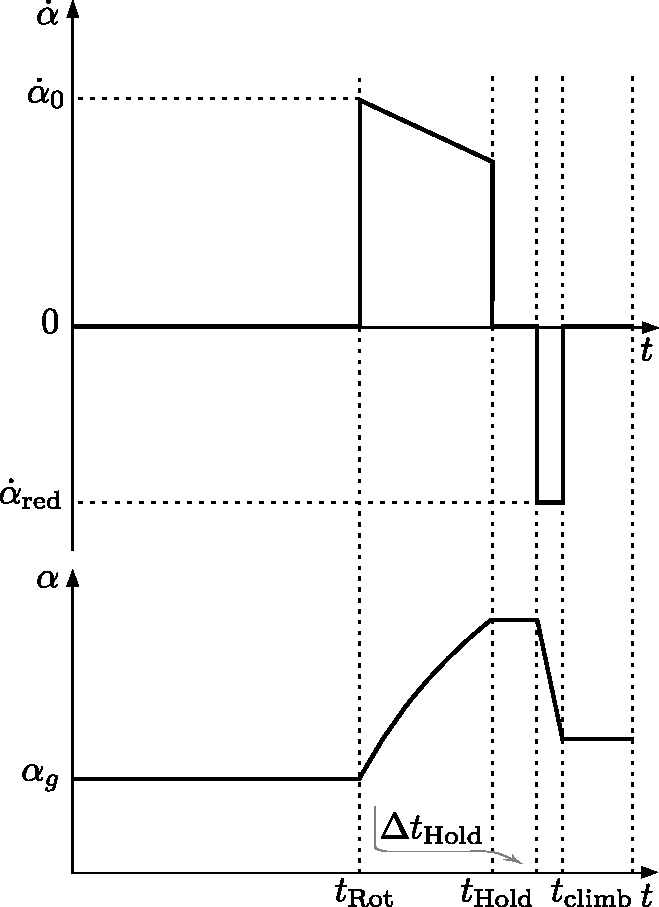
\includegraphics[keepaspectratio, width=0.45\textwidth]{AlphaInputTakeOff}
\caption{Qualitative representation of the angle of attack input law}
\label{fig:AlphaInput}
\end{figure}

\noindent
Figure~\ref{fig:AlphaInput} shows a qualitative representation of the $\alpha_1(t)$ law. As can be seen, after $t_{\text{Rot}}$ the pilot applies an initial angular velocity $\dot\alpha_{0}$, which decreases with time, according to the law written in (\ref{eqn:AlphaDot}) as function of $\alpha$, until the time $t_{\text{Hold}}$ has been reached; this particular instant is related to the achievement of the maximum admitted lift coefficient in take-off, which is set at 90\% of the $C_{L\text{max,TO}}$.

\begin{equation}
\dot\alpha=\dot\alpha_0\ \left(1-k_\alpha\ \alpha\right)
\label{eqn:AlphaDot}
\end{equation}

In equation (\ref{eqn:AlphaDot}), the $k_\alpha$ slope is assigned (a good value could be 0.07 ($\si{1/\degree}$)), while the initial angular velocity $\dot\alpha_0$ is calculated as follows.

\begin{equation}
\dot\alpha_0=\dfrac{\upDelta\alpha}{\upDelta t_{\text{Rot}}}=\dfrac{\alpha_{\text{LO}}-\alpha_g}{\upDelta t_{\text{Rot}}}
\label{eqn:AlphaDotInitial}
\end{equation}

where $\alpha_{\text{LO}}$ can be obtained from the lift curve of the wing, with flaps deflected in take-off configuration, by assigning the $C_{\text{L}_{\text{LO}}}$; this can be derived from the $C_{L\text{max,TO}}$ dividing it by the parameter $K^2_{\text{LO}}$, which represents the quantity that has to be multiplied by $V_{\text{S}}$ in order to obtain $V_{\text{LO}}$ (for example 1.1 with reference to table~\ref{tab:Take:Off:Speeds:FAR25}).

\bigskip
\noindent
From this point on the pilot stops the pitching manouver and keeps the angle of attack constant for an assigned $\upDelta t_{\text{Hold}}$. During this time interval, the lift coefficient is high and, as a result, also the induced drag is high so that aircraft acceleration will reduce. 

After this short time interval the pilot has to reduce the angle of attack in order to avoid the acceleration to decrease too much and so an assigned negative angular velocity $\dot\alpha_{\text{red}}$ is applied; the latter assumed to be constant for simplicity. 

Finally, since the decrease of $\alpha$ determines also a reduction in $C_L$, the time $t_{\text{climb}}$ will be reached when the load factor is reduced to 1; this means that a balance of the forces, perpendicular to the flight path, has been achieved and so the climb phase, at constant $\gamma$, can begin, leaving $\alpha$ constant and equal to last value reached. 

%-----------------------------OEI Take-Off subsection-----------------------------
\subsection{\gls{acr:OEI} take-off run and balanced field lenght}


%------------------------- JAVA CLASS ARCHITECTURE ---------------------------
\section{Java class architecture}
%----------------------- CASE STUDY : ATR72 AND B747 -------------------------
\section{Case study: B747-100B}
